\documentclass[12pt]{article}

\usepackage[utf8]{inputenc}
\usepackage[T1]{fontenc}
\usepackage{geometry}
\usepackage{graphicx} %figures
\usepackage{subfig} %subfigures
\usepackage{gensymb} %degree sign
\usepackage{amsmath} %math stuff
\usepackage{bm} %bold stuff
\usepackage[]{algorithm2e} %algorithms
\geometry{a4paper}

\title{Part 13: Multi-Objective Optimization}

\begin{document}
\date{March 1, 2021}
\maketitle

Hey everyone. Sorry for the week delay in the post, I wasn't totally happy with the result from looking at this stuff for only a week so this is a two week project. We are talking about multi-objective optimization (MOO), where we want to optimize over multiple potentially competing objectives $Y$ for given inputs $X$. First we'll talk about turning multiple objectives into a single objective (to abrogate the question of multiple objectives altogether), then we'll discuss more advanced topics like the famous NSGA-II algorithm and hypervolume maximization. 

\section{Multiple Outputs to Single Outputs}

\subsection{Linear Approach}

One way to approach MOO to the turn the various objectives into a single objective $\alpha$ that captures the design needs of the engineer. Perhaps the simplest version of this doesn't have a name but given objectives $Y_1$ and $Y_2$ we can get a single objective:

\begin{align*}
\alpha(x)=\beta\bar{Y_1}+(1-\beta)\bar{Y_2}
\end{align*}

\vspace{5mm}

Where $\bar{Y}$ indicates some kind of normalization (perhaps between $[0,1]$) and $\beta\in \rm I\!R$. Of course the larger $\beta$ the more $Y_1$ is emphasized in the optimization. We will use the \emph{BraninCurrin} function from the \emph{botorch} python toolbox, which is a $p=2$ input and $p_y=2$ output dimensional nonlinear design system shown in Figure 1a and 1d. If you want to optimize multiple objectives then maximize (or minimize) $\alpha$.

\vspace{5mm}

If we normalize $Y_1$ and $Y_2$ into $\bar{Y_1}$ and $\bar{Y_2}$ and use $\beta=\{0.25,0.5,0.75\}$ to show the effect of changing the emphasis of each output we get Figure 1. Note that the optimal point moves from $(x_1,x_2)=(1,0)$ to $(x_1,x_2)=(0.8,0.1)$ as $\beta$ increases (more emphasis on $Y_1$).

\vspace{5mm}

\begin{figure}[h]
\centering
\subfloat[][$\beta = 0 \: (Y_2) $]{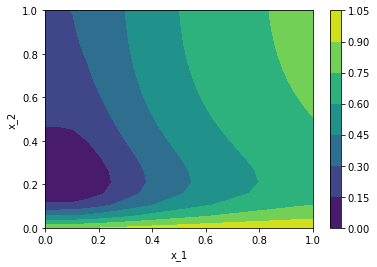
\includegraphics[width=0.2\textwidth]{Post_13_beta1}}
\subfloat[][$\beta = 0.25$]{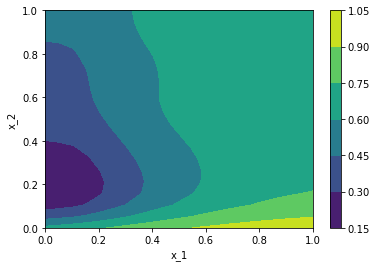
\includegraphics[width=0.2\textwidth]{Post_13_beta2}}
\subfloat[][$\beta = 0.50$]{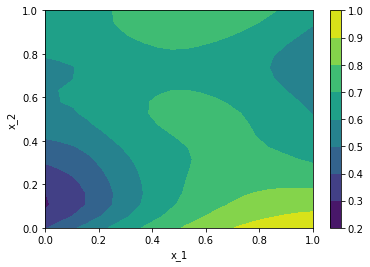
\includegraphics[width=0.2\textwidth]{Post_13_beta3}}

\subfloat[][$\beta = 0.75$]{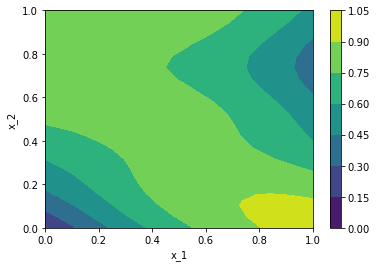
\includegraphics[width=0.2\textwidth]{Post_13_beta4}}
\subfloat[][$\beta = 1 \: (Y_1) $]{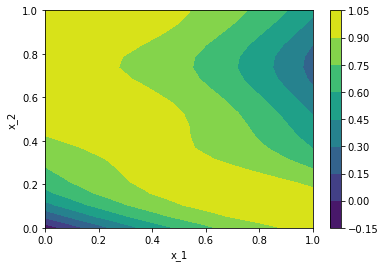
\includegraphics[width=0.2\textwidth]{Post_13_beta5}}
\caption{Plot of $\alpha$ for $\alpha(x)=\beta\bar{Y_1}+(1-\beta)\bar{Y_2}$}
\end{figure}

\vspace{5mm}

\subsection{Desirability Function Approach}

The next way of turning multiple outputs into a single objective is to calculate a \emph{desirability function}, where $Y_1$ and $Y_2$ are turned into a single $\alpha$ based on ranking parameters $w$ and shape parameters $r$ for outputs $j ... p_y$:

\begin{align*}
\alpha(x)=(\Pi_j^pd_j^{w_j})^{(\Sigma_j^pw_j)^{-1}}
\end{align*}

\begin{align*}
d_j=(\dfrac{Y_j-l_j}{u_j-l_j})^{r_j}
\end{align*}

\vspace{5mm}

Note that this just normalizes $Y_j$ to the upper $u_j$ and lower $l_j$ bounds of the output space $[0,1]$ and raises this to a power $r$ where the larger this shape factor the more extreme $d_j$ rises in the face of larger $Y_j$. Here is a plot of what $d_j$ looks like for various $r$ values. Each $Y_j$ is scaled by calculating $d_j$, which is combined by the weighted product of the functions. This forces $\alpha \rightarrow 0$ if any $d_j=0$. 

\vspace{5mm}

For Figure 2a I have added an additional constraint where the function changes to the upper $u_j$ and lower $l_j$ bounds if some effective upper and lower bound is reached (in this case 0.1 and 0.9). This shows how flexible this approach is. As an example, we recompute the \emph{BraninCurrin} function using the "Larger-The-Better" Desirability Function from \emph{Derringer and Suich} in Figure 2b.

\vspace{5mm}

When it comes to differentiation:

\begin{align*}
\dfrac{\partial\alpha(x)}{\partial x}=(\Pi_j^pd_j^{w_j})(\Sigma_j^p\dfrac{(d_j^{w_j})'}{d_j^{w_j}})
\end{align*}

\begin{align*}
(d_j^{w_j})'=\dfrac{w_j r (d_j)^{w_j-1}}{u_j-l_j} (\dfrac{y_j(x)-l_j}{u_j-l_j})^{r-1} \dfrac{\partial y_j(x)}{\partial x} 
\end{align*}

\vspace{5mm}

Which can be used in any gradient or Hessian-based method (I do not show a Hessian matrix because I don't hate my life and L-BFGS-B which we'll hopefully do an entire post about). For Figure 2a the discontinuities may be solved for using a sub-differential modification to the above gradient.

\begin{figure}[h]
\centering
\subfloat[][Example $d_j$ Component Function for Different $r$]{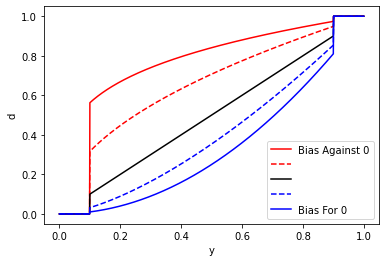
\includegraphics[width=0.5\textwidth]{Post_13_des}}
\subfloat[][Contour of \emph{BraninCurrin}]{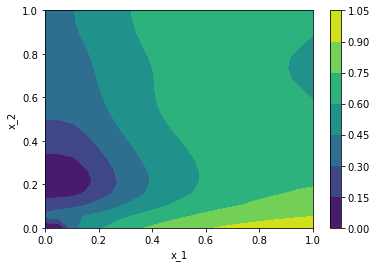
\includegraphics[width=0.5\textwidth]{Post_13_des_contour}}
\caption{"Larger-The-Better" Desirability Function from \emph{Derringer and Suich} | for the right plot $r=\{1,1\}$ and $w=\{1,2\}$ indicating linear regime and higher weighting to $Y_2$}
\end{figure}

\section{NSGA-II Approach}

One popular method for optimization is the NSGA-II algorithm; a genetic algorithm meant to search for "pareto" solutions (where improving one output reduces quality for one or more other outputs) to the function while maintaining a degree of separation between solutions. This method is very generalizable because (i) it doesn't require the user to specify their opinion of the solution (such as with the linear or desirability function approach) and (ii) is a genetic algorithm so doesn't need derivatives to solve for optimal points.

\vspace{5mm}

The NSGA-II algorithm is similar to the typical genetic algorithm discussed in the previous post and follows this structure:

\begin{itemize}
	\item Rank $2N$ solutions by their pareto rank (i.e. how many other solutions they dominate).
	\item Allow the best solutions (with highest pareto rank) to be selected for crossover and mutation.
	\item Also allow some solutions not pareto dominant to be selected for crossover and mutation based on their distance from other points.
\end{itemize}

The actual implementation of this is a bit of a pain to explain, so I'll refer you to the famous \emph{Deb et al} paper, the python implementation \emph{pymoo}, and my code. Note that in the python code, my distance operator is simpler than Deb's. From Figure 3 it's clear that NSGA-II is pretty good at replicating the \emph{BraninCurrin} pareto front (for maximization).

\vspace{5mm}

I want to make it clear that NSGA-II really is the workhorse for MOO problems. It comes up everywhere and is super applicable. One drawback is that it requires a lot of data (or approximations of the true data) because it is a genetic algorithm.

\begin{figure}[h]
\centering
\subfloat[][NSGA-II]{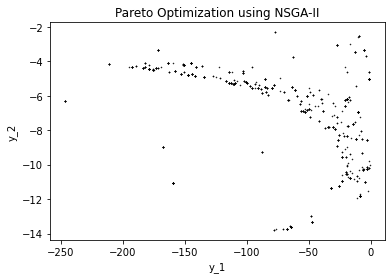
\includegraphics[width=0.45\textwidth]{Post_13_nsgaii}}
\subfloat[][Random Sample of \emph{BraninCurrin}]{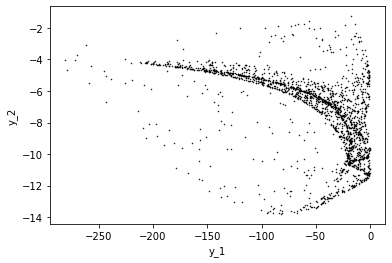
\includegraphics[width=0.45\textwidth]{Post_13_bc}}
\caption{Pareto of \emph{BraninCurrin}}
\end{figure}

\section{Hypervolume Optimization}

Speaking of large data requirements, the gaussian process-aided hypervolume optimization method is a popular way of solving MOO problems with little data. The idea is that, relative to some points $Y_{ref}$, the geometric shape between the previous pareto front and the current front is the hypervolume improvement. With a gaussian process this is further aided with uncertainty bands (because gaussain processes give means $\mu$ and standard deviations $\sigma$). 

\vspace{5mm}

This can be considered a bayesian optimization problem because we have an objective function $\alpha$ which has uncertainty. In Figure 4b I have shown the result of the code where, given $N=10$ datapoints, we use q-HVEI (q-Hypervolume Expected Improvement) to solve for $q=2$ most optimal points to sample. Note that the result looks pitiful compared to NSGA-II, but remember the NSGA-II had access to the underlying \emph{BraninCurrin}, while this q-HVEI only had $N=10$ points available. Not bad!

\begin{figure}[h]
\centering
\subfloat[][Hypervolume Improvement Function]{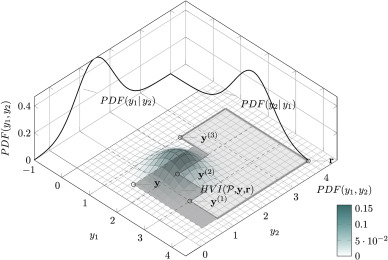
\includegraphics[width=0.5\textwidth]{Post_13_hypervolume}}
\subfloat[][q-Hypervolume Improvement for \emph{BraninCurrin} where $q=2$]{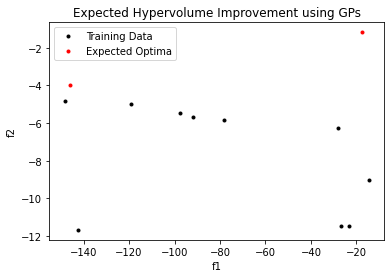
\includegraphics[width=0.5\textwidth]{Post_13_hypervolumeBO}}
\caption{\textbf{left} from \emph{Yang et al 2019} paper and \textbf{right} red = $q$ suggested query points, black = current data}
\end{figure}

\vspace{5mm}

Thanks for the patience everyone! Sorry this took so long to post. This is by no means an exhaustive list of MOO methods, but is a pretty good primer and even goes into some detail especially if you dig into the code. Next week I'd like to take it a bit easy so we're going to implement our own \emph{gyptorch} kernel!

\end{document}